\chapter{Космические корабли и станции: современные реалии 50-летней давности}
\label{ch:spacecraft-space-station}

\begin{marginfigure}[16\baselineskip]
    \MarginQuestion
    В какой стране спроектирован этот аппарат?

    \vspace{3pt}
	\includegraphics[width=0.43\linewidth]{graphics/chapter/spacecraft_space_station/soyuz-19.jpg}

    См. ответ~\ref{answer:spacecraft_USSR} на с.~\pageref{answer:spacecraft_USSR}\\
    \label{question:spacecraft_soyuz19}
\end{marginfigure}

Глава посвящена исследованию космических кораблей и станций на основе Викиданных. 
С~помощью SPARQL-скриптов построен список отечественных кораблей и станций, 
нарисованы временные графики запуска кораблей в нашей стране и в мире за период с 1960 по 2021 год. 
Выполнена оценка полноты Викиданных, показавшая, 
что многие объекты имеют неправильное значение свойства \wdProperty{31}{частный случай понятия}\footnote{%
    <<Частный случай понятия>> или <<экземпляр>> 
    (англ. \emph{instance of})~--- это конкретный объект класса, категории, 
    одно из основных свойств (отношений), используемых в Викиданных и позволяющих классифицировать объекты, 
    соотносить их разным <<классам>>, <<категориям>>.%
}. 
В ходе работы было обнаружено, что текущие показатели росийской космонавтики по количеству запусков космических кораблей за последние годы соответствуют показателям в СССР пятьдесят лет назад. 



\section{Список космических кораблей и станций}

Построим запрос~\ref{lst:spaceships} для вывода списка всех космических кораблей и станций. 
Нам потребуются объекты \wdqName{космическая станция}{25956}, 
\wdqName{космический корабль}{40218} и отношение \wdProperty{31}{экземпляр}. 

\index{SPARQL!VALUES!Список кораблей и станций}
\index{SPARQL!SERVICE!Список кораблей и станций}
\begin{lstlisting}[ language=SPARQL, numbers=none, caption={{\href{https://w.wiki/4d4f}{Список кораблей и станций}}\protect\footnotemark}, label=lst:spaceships, ]
# List of spacecraft (Q40218) and space station (Q25956)
SELECT  ?s ?sLabel ?typeLabel WHERE {
  VALUES ?type {wd:Q40218 wd:Q25956}
  ?s wdt:P31 ?type.  # Selecting the type of object
  SERVICE wikibase:label {bd:serviceParam wikibase:language"ru,en"}
}
\end{lstlisting}
\footnotetext{Получено: 145 объектов в 2021 году. SPARQL-запрос: \mbox{\url{https://w.wiki/4d4f}}.}


\section{Глубина проработки объектов}


Сервис ProWD показал\autocite{spacecraftProWD}, что заполнение космических объектов неравномерное, 
большая часть заполнена менее чем на 30\,\%. 
По состоянию на 2021 год наиболее полным и проработанным в~Викиданных 
является космический корабль \wdqName{Аполлон-8}{184201}, 
имеющий 30 свойств\autocite{spacecraftProWD}. 
При этом всего по одному свойству имеют такие корабли, как\autocite{spacecraftProWD}:
\begin{compactitemize}
    \item \wdqName{Europa Astrobiology Lander}{10491365}, 
    \item \wdqName{Project Orbiter}{6514453}, 
    \item \wdqName{LRK}{5961734}, 
    \item \wdqName{EarthForce One}{5327028}\sidenote[][]{%
%
Отметим непростую судьбу объекта \wdqName{EarthForce One}{5327028}. 
Этот объект был создан в Викиданных ботом автоматически в 2013 году, 
поскольку существовала статья в Английской Википедии \href{https://en.wikipedia.org/wiki/EarthForce_One}{EarthForce One}. 
Статья была удалена из-за~отсутствия надёжных источников, 
доказывающих значимость объекта, 
а~в~Викиданных объект остался как неприкаянный. 
Подумайте над запросом, который вывел бы список аналогичных объектов Викиданных, 
не соответствующих ни одной статье Википедии.%
%
}, 
    \item \wdqName{Союз ГВК}{60767924}, 
    \item \wdqName{CubeSat for Solar Particles}{22907583}. 
\end{compactitemize}



\section{Список отечественных кораблей и станций}

\begin{marginfigure}[0\baselineskip]
    \MarginQuestion
    В какой стране спроектирован этот аппарат?

    \vspace{3pt}
	\includegraphics[width=0.43\linewidth]{graphics/chapter/spacecraft_space_station/soyuz-t.jpg}

    См. ответ~\ref{answer:spacecraft_USSR} на с.~\pageref{answer:spacecraft_USSR}\\
    \label{question:spacecraft_soyuzT}
\end{marginfigure}

Найдём корабли и станции, сконструированные в СССР или России, 
с помощью запроса~\ref{lst:spaceshipsUSSR}.

\index{SPARQL!SERVICE!Список отечественных кораблей}
\begin{lstlisting}[ language=SPARQL, 
                    numbers=none, 
                    caption={{\href{https://w.wiki/4d9c}{Список отечественных кораблей}}\protect\footnotemark}, 
                    label=lst:spaceshipsUSSR
                  ]
# List of Russian and USSR spacecrafts and stations
SELECT  ?spacecraft  ?spacecraftLabel WHERE
{
  {?spacecraft wdt:P31 wd:Q40218.} UNION #spacecraft
  {?spacecraft wdt:P31 wd:Q25956.} # and space station
  
  # Soviet Union and Russia
  VALUES ?ruCountries {wd:Q15180 wd:Q159}
  ?spacecraft wdt:P17 ?ruCountries. # related to Russian countries
  
  SERVICE wikibase:label {bd:serviceParam wikibase:language "ru,en"}
}
\end{lstlisting}
\footnotetext{Получено: 3 отечественных корабля и станции 
в~2017~году и 25~--- в~2021 году. SPARQL-запрос: \href{https://w.wiki/4BbY}{https://w.wiki/4d9c}.}



\section{Анализ полноты Викиданных}

Проанализируем степень заполнения Викиданных в области отечественных космических кораблей и станций. 
Если по запросу~\ref{lst:spaceships} было получено 145 кораблей и станций во всём мире, 
то~по~запросу~\ref{lst:spaceshipsUSSR}~--- всего 25 отечественных объектов. 
Информации о~советских и российских объектах в 2021 году 
стало в несколько раз больше по сравнению с 2017 годом, 
когда по запросу~\ref{lst:spaceshipsUSSR} выдавалось всего 3 объекта. 

На сайте Буран.ру в разделе о космических кораблях СССР и России на 2021 год 
содержится информация о 36 кораблях\autocite{spacecraftBuran}. 
В советской энциклопедии <<Космонавтика>> от 1985 года упоминаются 
94 космических корабля и орбитальных станции СССР и США, 
запущенных с 1961 по 1983 год, 
из~них 51 корабль принадлежит СССР\autocite[498]{spacecraftCosmonavtika}. 
Это означает, что в Викиданных представлено менее половины советских космических кораблей. 
В американском справочнике по космонавтике и астрономии 
приведены 10 советских и российских запусков космических станций\autocite[296]{spacecraftSAA}, 
126 запусков шаттла НАСА с 1981 по 2008 год\autocite[288]{spacecraftSAA} 
и характеристики 31 ракеты-носителя\autocite[290--291]{spacecraftSAA}. 




\section{Временные графики освоения космоса в~нашей стране и мире}


\begin{marginfigure}[0\baselineskip]
    \MarginQuestion 
    \index{SPARQL!квалификатор!of}
    В предыдущих запросах мы искали экземпляры космических кораблей, 
    то~есть искали в~Викиданных утверждения ``is instance of spacecraft''. 
    На рисунке ниже показан вариант утверждения 
    о~космических кораблях, входящих в~какую-либо линейку, а~именно: 
    ``is instance of product model of spacecraft''. 
    Когда есть линейка моделей, в нашем случае~--- серия космических кораблей, 
    тогда нужен объект \wdqName{product model}{10929058}. 
    На~рисунке of и spacecraft~--- 
    это соответственно свойство и значение квалификатора, характеризующего объект \emph{product model} 
    (см.~справку Викиданных \href{https://www.wikidata.org/?curid=16567549}{Help:Квалификаторы}). 
    Найдите серии космических кораблей с~использованием квалификаторов. 

    \vspace{3pt}
	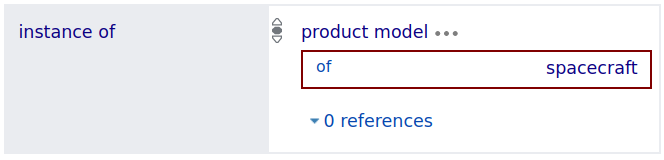
\includegraphics[width=0.8\linewidth]{graphics/chapter/spacecraft_space_station/is_product_model_red.png}

    См. ответ на с.~\pageref{answer:product_model}\\
    \label{question:product_model}
\end{marginfigure}
%    для серии космических кораблей \wdqName{Союз 7К-Л1}{1959194}. 


Временной (с 1960-х годов) 
график запуска космических аппаратов в нашей стране (рис.~\ref{fig:launchesRussia5years}) 
построен с помощью запроса~\ref{lst:launchesRussia5years}.%

Ранее в запросах для получения каких-либо списков мы использовали свойство \wdProperty{31}{экземпляр}. 
В запросе~\ref{lst:launchesRussia5years} мы обошлись без этого свойства за счёт использования отношения 
\wdProperty{619}{<<дата запуска космического корабля>>} в строке 10 
для обхода и подсчёта таких объектов, которые были запущены в космос.  

Логический оператор \lstinline|UNION| в строках 5--8 
позволяет объединить советские и российские запуски космолётов. 

Если бы в запросе~\ref{lst:launchesRussia5years} 
вместо переменной \lstinline|?lapse| оставалась~--- \lstinline|?year| (строки 3 и 12), 
то~мы~получили бы на рис.~\ref{fig:launchesRussia5years} 
число запусков за каждый год. 
Благодаря функции округления \mbox{\lstinline|FLOOR()|} 
и оператору \lstinline|GROUP| выполняется группировка%
%
\sidenote[][]{
%
        В строке 15 запроса~\ref{lst:launchesRussia5years} 
        запущенные в космос объекты группируются командой: 
        \mbox{\lstinline|GROUP BY ?lapse|.} 
        То, что группировка идёт именно по~пятилеткам, а~не,~например шестилеткам, 
        определяется в строке 12, где переменная \lstinline|?year| делится на 5, округляется, умножается на 5.%
} 
 кораблей, запущенных в~течение пяти лет. 
При~этом~в~переменную \lstinline|?quantity| записывается число этих объектов за~пятилетку, 
подсчитанное с помощью функции \lstinline|COUNT()|.

Для представления результатов в виде столбчатой диаграммы используется стиль отображения BarChart 
(см. вторую строку запроса~\ref{lst:launchesRussia5years}).




\begin{figure*}[h!]
    \index{График!BarChart!Запуски космических кораблей в России}
    \includegraphics[width=\linewidth]{graphics/chapter/spacecraft_space_station/Visualization of the number of spacecraft launches in USSR and Russia per 5 years 2022.png}
    \caption[График запусков космических кораблей в СССР и России, 2022 год.]{Диаграмма количества запусков космических кораблей в СССР и России по пятилеткам}%
    \label{fig:launchesRussia5years}%
\end{figure*}



\newpage\phantom{blabla}

Горизонтальной ос\'{и} на рис.~\ref{fig:launchesRussia5years} 
отвечает переменая \mbox{\lstinline|?lapse_str|} в~запросе~\ref{lst:launchesRussia5years}. 
Если не преобразовывать число \lstinline|?lapse| 
в текстовую переменную \mbox{\lstinline|?lapse_str|}%
\sidenote[][]{
%
        Преобразование числа в текст  
        в третьей строке запроса~\ref{lst:launchesRussia5years}:\newline
        \lstinline|(STR(?lapse) AS ?lapse_str)|.%
%
}, то ось~X имеет диапазон от 0 до 2200 
вместо требуемого диапазона от 1960 до 2025 года, 
а~результаты обозначаются точками с~координатами (пятилетка, число запусков), 
в~итоге график становится нечитаемым. 

На рис.~\ref{fig:launchesRussia5years} видно, 
что самый активный период развития отечественной космонавтики был в~1970--1995 годах.



\newpage

%%%%%%%%%%%%%%%% Упражнение 1 %%%%%%%%%%%%%%%% 
\marginnote[2cm]{
        \label{question:spacecraft_1}
        \MarginQuestion
        Сколько кораблей было запущено в~СССР в~1960-е, 1970-е и 1980-е годы?

        См. ответ~\ref{answer:launches_USSR} на с.~\pageref{answer:launches_USSR}.%
}

\index{SPARQL!STR!Запуски космических кораблей в России}
\index{SPARQL!BIND!Запуски космических кораблей в России}
\index{SPARQL!YEAR!Запуски космических кораблей в России}
\index{SPARQL!FLOOR!Запуски космических кораблей в России}
\index{SPARQL!UNION!Запуски космических кораблей в России}
\index{SPARQL!COUNT!Запуски космических кораблей в России}
\index{SPARQL!GROUP BY!Запуски космических кораблей в России}
\index{SPARQL!ORDER BY!Запуски космических кораблей в России}
\begin{lstlisting}[ language=SPARQL, 
    caption={{\href{https://w.wiki/4eGg}{Запуски космических кораблей в СССР и России}}\protect\footnotemark}, 
    label=lst:launchesRussia5years,
    texcl
                  ]
# The number of spacecraft launches in Russia every 5 years
#defaultView:BarChart
SELECT (STR(?lapse) AS ?lapse_str) (COUNT(?item) AS ?quantity)
WHERE {                                  # spacecraft belongs to
        {?item wdt:P17 wd:Q15180}               # country = USSR
  UNION {?item wdt:P17 wd:Q159}               # country = Russia
  UNION {?item wdt:P495 wd:Q159}    # country of origin = Russia
  UNION {?item wdt:P495 wd:Q15180}.  # country of origin =  USSR
  
  ?item wdt:P619 ?launch. # date of spacecraft launch
  BIND( YEAR(?launch) AS ?year) 
  BIND(FLOOR(?year/5)*5 AS ?lapse) # count for each 5 years
SERVICE wikibase:label {bd:serviceParam wikibase:language "ru,en"}
} 
GROUP BY ?lapse
ORDER BY ?lapse # Order 1970, 1975, 1980, ...
\end{lstlisting}
\footnotetext{Получено: 14 пятилеток. SPARQL-запрос: \href{https://w.wiki/4eGg}{https://w.wiki/4eGg}.}
%\marginnote[0cm]{Найдено 14 пятилеток. SPARQL-запрос: \href{https://w.wiki/4eGg}{https://w.wiki/4eGg}} 



\index{SPARQL!COUNT!Запуски космических кораблей в мире}
\index{SPARQL!YEAR!Запуски космических кораблей в мире}
\index{SPARQL!BIND!Запуски космических кораблей в мире}
\index{SPARQL!SERVICE!Запуски космических кораблей в мире}
\index{SPARQL!GROUP BY!Запуски космических кораблей в мире}
\begin{lstlisting}[ language=SPARQL, 
                    numbers=none, 
                    caption={{\href{https://w.wiki/4bEu}{Запуски космических кораблей в мире по годам и странам}}\protect\footnotemark}, 
                    label=lst:launchesWorld
                  ]
#defaultView:BarChart
SELECT ?year (COUNT(?obj) AS ?count) ?country ?countryLabel WHERE {
  ?obj wdt:P17 ?country. # spacecraft belongs to country 
  ?obj wdt:P619 ?launch. # date of spacecraft launch
  BIND(str(YEAR(?launch)) AS ?year)
  SERVICE wikibase:label {bd:serviceParam wikibase:language "ru,en"}
}
GROUP BY ?year ?country ?countryLabel
\end{lstlisting}
\footnotetext{Получено: 328 результатов в 2021 году. Ссылка на SPARQL-запрос: \href{https://w.wiki/4bEu}{https://w.wiki/4bEu}.}



Запрос~\ref{lst:launchesWorld} строит график 
запусков космических кораблей в~мире по~годам и странам. 
Рис.~\ref{fig:launchesWorld} показывает, что больше всего космических аппаратов 
запускали Индия и США 
(только у них зафиксировано более 10 ежегодных запусков) в 2017--2018 годах. 
Пик запусков в мире был в 2018 году (59 запусков). 




\newpage

\index{График!BarChart!Запуски космических кораблей по годам и странам}
\begin{figure*}[h!]
  \includegraphics[width=\linewidth]{graphics/chapter/spacecraft_space_station/Visualization of the number of spacecraft launches by year and country 2021.png}
  \caption[График запусков космических кораблей в мире по годам и странам, 2021 год.]{Диаграмма ежегодного суммарного количества запусков космических кораблей по всем странам}
  \label{fig:launchesWorld}%
\end{figure*}


\newpage

%%%%%%%%%%%%%%%% Упражнение 2 %%%%%%%%%%%%%%%% 
\marginnote[6\baselineskip]{%
        \label{question:spacecraft_2}
        \MarginQuestion
        Какое наибольшее и наименьшее количество запусков космических кораблей за~десятилетие совершило человечество с~1970 по~2010 год?

        См. ответ~\ref{answer:max-min-space-launches} на с.~\pageref{answer:max-min-space-launches}.
}
По Викиданным, российская космонавтика занимает средние позиции по количеству запусков, 
её численные показатели за 2016--2019 годы схожи с показателями СССР в 1970-е и 1980-е годы 
и составляют 3--5 запусков в год.



\section{Космонавты в международных полётах}

Запрос~\ref{lst:internationalFlights} строит граф~\ref{fig:internationalFlights} 
c~вершинами типа <<ракеты>> и <<космонавты>> с~раскраской по~странам.

\index{SPARQL!DISTINCT!Космонавты в международных полётах}
\index{SPARQL!SERVICE!Космонавты в международных полётах}
\index{SPARQL!BIND!Космонавты в международных полётах}
\index{SPARQL!VALUES!Космонавты в международных полётах}

\footnote[17][2\baselineskip]{Получено: 68 результатов в 2022 году. Ссылка на SPARQL-запрос: \href{https://clck.ru/agioQ}{https://clck.ru/agioQ}.}
\begin{lstlisting}[ language=SPARQL, caption={{\href{https://clck.ru/agioQ}{Космонавты в международных полётах}}\protect\footnotemark}, 
                    label=lst:internationalFlights
                  ]
# Graph of astronauts as crew of flights of different countries
#defaultView:Graph
SELECT DISTINCT ?item ?itemLabel ?rgb ?link ?naut_seed
WHERE
{ 
  VALUES ?toggle { true false }
  # Let's select a subset of astronauts
  {
    SELECT DISTINCT ?naut WHERE
    { 
      VALUES ?naut_seed {wd:Q313815}.  # Sergei Krikalev
      ?s wdt:P1029 ?naut_seed, ?naut;  
    }       # ?naut_seed & ?naut are member of a same crew
  }
  ?s  wdt:P31/wdt:P279* wd:Q40218; # spacecraft and subclasses
      wdt:P31/wdt:P279* wd:Q752783;# human spaceflight and subclasses
          wdt:P1029 ?naut;         # has member of the crew ?naut    
  SERVICE wikibase:label {bd:serviceParam wikibase:language "ru,en"}
  BIND(IF(?toggle,?s,?naut) AS ?item).
  BIND(IF(?toggle,?sLabel,?nautLabel) AS ?itemLabel).
  BIND(IF(?toggle,"FFFFFF","7FFF00") AS ?rgb_source).
  BIND(IF(?toggle,"",?s) AS ?link).
  ?naut wdt:P27 ?country. # astronaut is citizen of country 
  # ?toggle = true then spacecraft node
  # ?toggle = false then astronaut node
  BIND(             # Soviet & Russian astronauts have red nodes
    IF(!?toggle && (?country=wd:Q15180||?country=wd:Q159),"FF0000",
    IF(!?toggle && ?country=wd:Q30,"FF00FF",  # USA - fuchsia
    IF(!?toggle && ?country=wd:Q183,"C0C0C0", # Germany - silver
    IF(!?toggle && ?country=wd:Q142,"008080", # France - teal
    IF(!?toggle && ?country=wd:Q40,"800000", # Austria - maroon
    IF(!?toggle && ?country=wd:Q38,"00FFFF", # Italy - aqua
    ?rgb_source))))))
    AS ?rgb).
}
\end{lstlisting}
%\footnotetext{Получено: 68 результатов в 2022 году. Ссылка на SPARQL-запрос: \href{https://clck.ru/agioQ}{https://clck.ru/agioQ}.}

Для работы скрипта необходимо указать начальную точку~--- космонавта, 
который принимал участие в международных космических полётах. 
Начальная точка задаётся в~строке~11 скрипта и записывается в переменную \lstinline|?naut_seed|. 
Далее, в~строке~12, выполняется поиск астронавтов, 
летавших совместно с тем, кого мы указали ранее. 
В~строках~15--17 подгружаются данные о космических аппаратах, полётах и астонавтах. 
Булева переменная \lstinline|?toggle| имеет значение \lstinline|?true|, 
если найденный объект является космическим аппаратом, 
или \lstinline|?false|, 
если найденный объект является космонавтом. 
В переменную \lstinline|?item| в строке 19 записывается выбранный объект (космический аппарат или космонавт). 
В~строке~20 в~переменную \lstinline|?itemLabel| записывается название объекта, 
в~строке~21 в~переменную \lstinline|?rgb_source| записываются данные для раскраски кораблей. 

Если выбран корабль, то в строке 22 в переменную \lstinline|?link| ничего не записывается, 
если выбран космонавт, то в переменную~\lstinline|?link| записываем его корабль. 
На графе (рис.~\ref{fig:internationalFlights}) этой переменной будет соответствовать дуга от космонавта к кораблю. 

В строке 23 подгружаются данные о гражданстве космонавта, 
а~в~строках 26--34 вершинам космонавтов на графе присваивается цвет в зависимости от их гражданства (рис.~\ref{fig:internationalFlights}). 



\section{Упражнения}
\begin{enumerate}
  \item Постройте список кораблей, которые отправились или отправятся на \wdqName{Марс}{111}.
  \item Подсчитайте долю кораблей (нарисуйте график по десятилетиям), 
        отправленных на \wdqName{Марс}{111}, 
        по отношению к числу кораблей, отправленных на \wdqName{Луну}{405}.
  \item Подсчитайте количество \wdqName{успешных}{7632586} космических запусков 
      относительно \wdqName{неудачных}{1121708}\sidenote[][-24pt]{%
%
Например, у объекта \wdqName{<<космическая программа Луна>>}{192372} 
в свойстве \wdProperty{793}{<<ключевое событие>>} 
указано число успешных и неудачных запусков.%
}.%
\end{enumerate}



\index{График!Graph!Космонавты в международных полётах}
\begin{figure*}[h]
%  \setlength{\fboxsep}{0pt}%
%  \setlength{\fboxrule}{1pt}%
%  \fcolorbox{gray}{gray}
  \caption[Ракеты и космонавты на графе, 2022 год.]{Фрагмент графа c вершинами типа <<ракеты>> и <<космонавты>> с~раскраской по~странам. Красный цвет соответствует СССР и России, розовый~--- США, серый~--- Германии, бирюзовый~--- Франции, бордовый~--- Австралии, а голубой~--- Италии}
  \label{fig:internationalFlights}%
\end{figure*}
